\documentclass[tikz,border=0pt]{standalone}
\usepackage{amsmath,amssymb}
\usepackage[scaled]{helvet}
\renewcommand{\familydefault}{\sfdefault}
\usetikzlibrary{arrows.meta,backgrounds,calc,fit,positioning,shapes.geometric}
\definecolor{bpink}{HTML}{172033}
\definecolor{bpblue}{HTML}{2A78D6}
\definecolor{bporange}{HTML}{E56A32}
\definecolor{bpgreen}{HTML}{168A65}
\definecolor{bppurple}{HTML}{7A5CC7}
\definecolor{bpred}{HTML}{C94A4A}
\definecolor{bpmuted}{HTML}{667085}
\definecolor{bpgrid}{HTML}{D8DEE8}
\definecolor{bpsurface}{HTML}{F8FAFC}
\tikzset{
  var/.style={circle,draw=bpblue,fill=bpblue!10,line width=.9pt,minimum size=8mm,font=\small\bfseries,text=bpink},
  factor/.style={rectangle,rounded corners=1.5pt,draw=bporange,fill=bporange!14,line width=.9pt,minimum size=6.8mm,font=\small\bfseries,text=bpink},
  constraint/.style={rectangle,rounded corners=1.5pt,draw=bpred,fill=bpred!12,line width=.9pt,minimum size=6.8mm,font=\small\bfseries,text=bpink},
  edge/.style={draw=bpmuted!75,line width=.9pt},
  msgvf/.style={-{Latex[length=2.2mm]},draw=bpblue,line width=1.35pt},
  msgfv/.style={-{Latex[length=2.2mm]},draw=bporange,line width=1.35pt},
  label/.style={font=\scriptsize,text=bpmuted,align=center},
  title/.style={font=\bfseries\large,text=bpink},
  card/.style={draw=bpgrid,fill=bpsurface,rounded corners=7pt,line width=.7pt},
}

\begin{document}
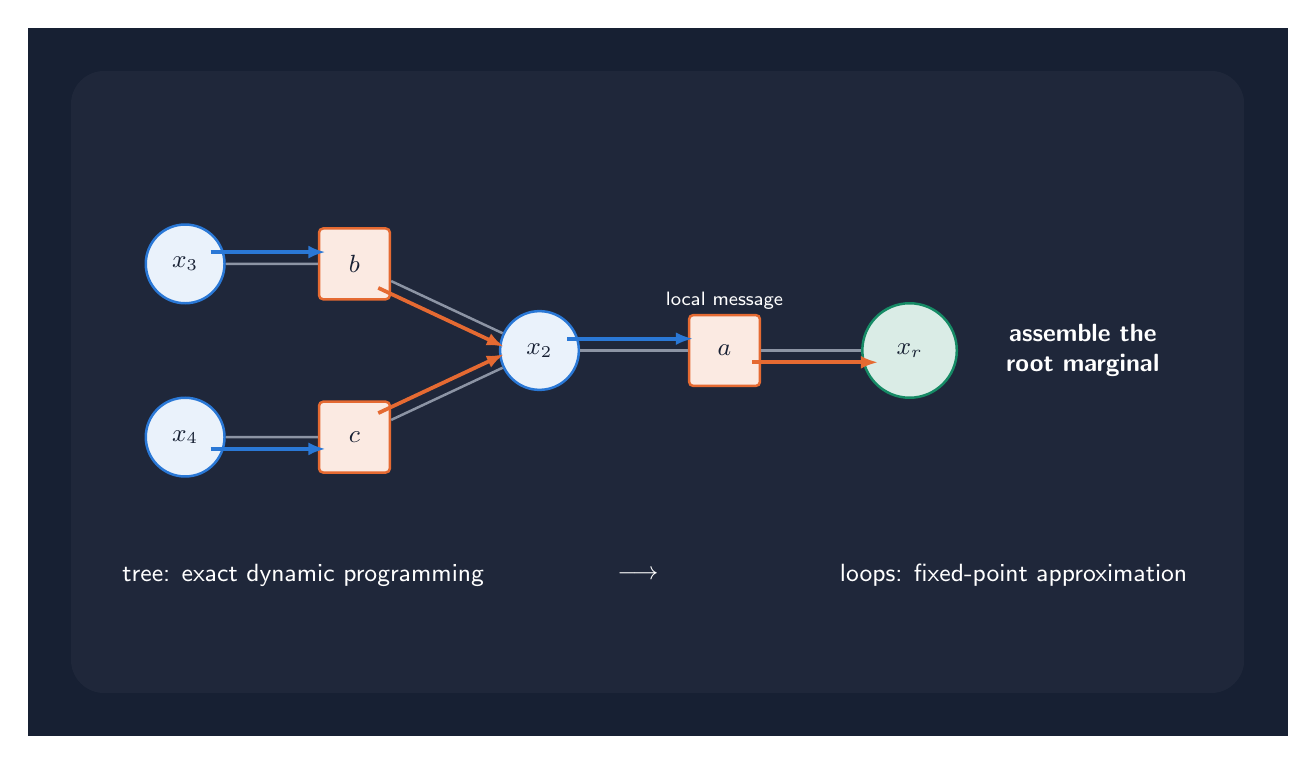
\begin{tikzpicture}[x=1cm,y=1cm,font=\sffamily]
  \path[use as bounding box] (0,0) rectangle (16,9);
  \fill[bpink] (0,0) rectangle (16,9);
  \fill[white,opacity=.035,rounded corners=12pt] (.55,.55) rectangle (15.45,8.45);
  \begin{scope}[yshift=0.35cm]
  \node[var,minimum size=10mm] (x3) at (2.0,5.65) {$x_3$};
  \node[var,minimum size=10mm] (x4) at (2.0,3.45) {$x_4$};
  \node[factor,minimum size=9mm] (b) at (4.15,5.65) {$b$};
  \node[factor,minimum size=9mm] (c) at (4.15,3.45) {$c$};
  \node[var,minimum size=10mm] (x2) at (6.5,4.55) {$x_2$};
  \node[factor,minimum size=9mm] (a) at (8.85,4.55) {$a$};
  \node[var,draw=bpgreen,fill=bpgreen!16,minimum size=12mm] (root) at (11.2,4.55) {$x_r$};
  \draw[edge] (x3)--(b)--(x2);
  \draw[edge] (x4)--(c)--(x2);
  \draw[edge] (x2)--(a)--(root);
  \draw[msgvf] ($(x3)!0.15!(b)+(0,.15)$) -- ($(x3)!0.83!(b)+(0,.15)$);
  \draw[msgfv] ($(b)!0.15!(x2)+(-.05,-.14)$) -- ($(b)!0.83!(x2)+(-.05,-.14)$);
  \draw[msgvf] ($(x4)!0.15!(c)+(0,-.15)$) -- ($(x4)!0.83!(c)+(0,-.15)$);
  \draw[msgfv] ($(c)!0.15!(x2)+(-.05,.14)$) -- ($(c)!0.83!(x2)+(-.05,.14)$);
  \draw[msgvf] ($(x2)!0.15!(a)+(0,.15)$) -- ($(x2)!0.83!(a)+(0,.15)$);
  \draw[msgfv] ($(a)!0.15!(root)+(0,-.15)$) -- ($(a)!0.83!(root)+(0,-.15)$);
  \node[text=white!72,font=\scriptsize] at (8.85,5.18) {local message};
  \node[text=white,font=\bfseries\small,align=center] at (13.4,4.55) {assemble the\\root marginal};
  \end{scope}
  \node[anchor=west,text=white!62,font=\small] at (1.08,2.05) {tree: exact dynamic programming};
  \node[text=white!35,font=\small] at (7.75,2.05) {$\longrightarrow$};
  \node[anchor=east,text=white!62,font=\small] at (14.85,2.05) {loops: fixed-point approximation};
\end{tikzpicture}
\end{document}
